% Copyright (c) 2015 Daniele Masini - d.masini.it@gmail.com

\chapter{Quadrilateri}\label{chap:quadrilateri}

% 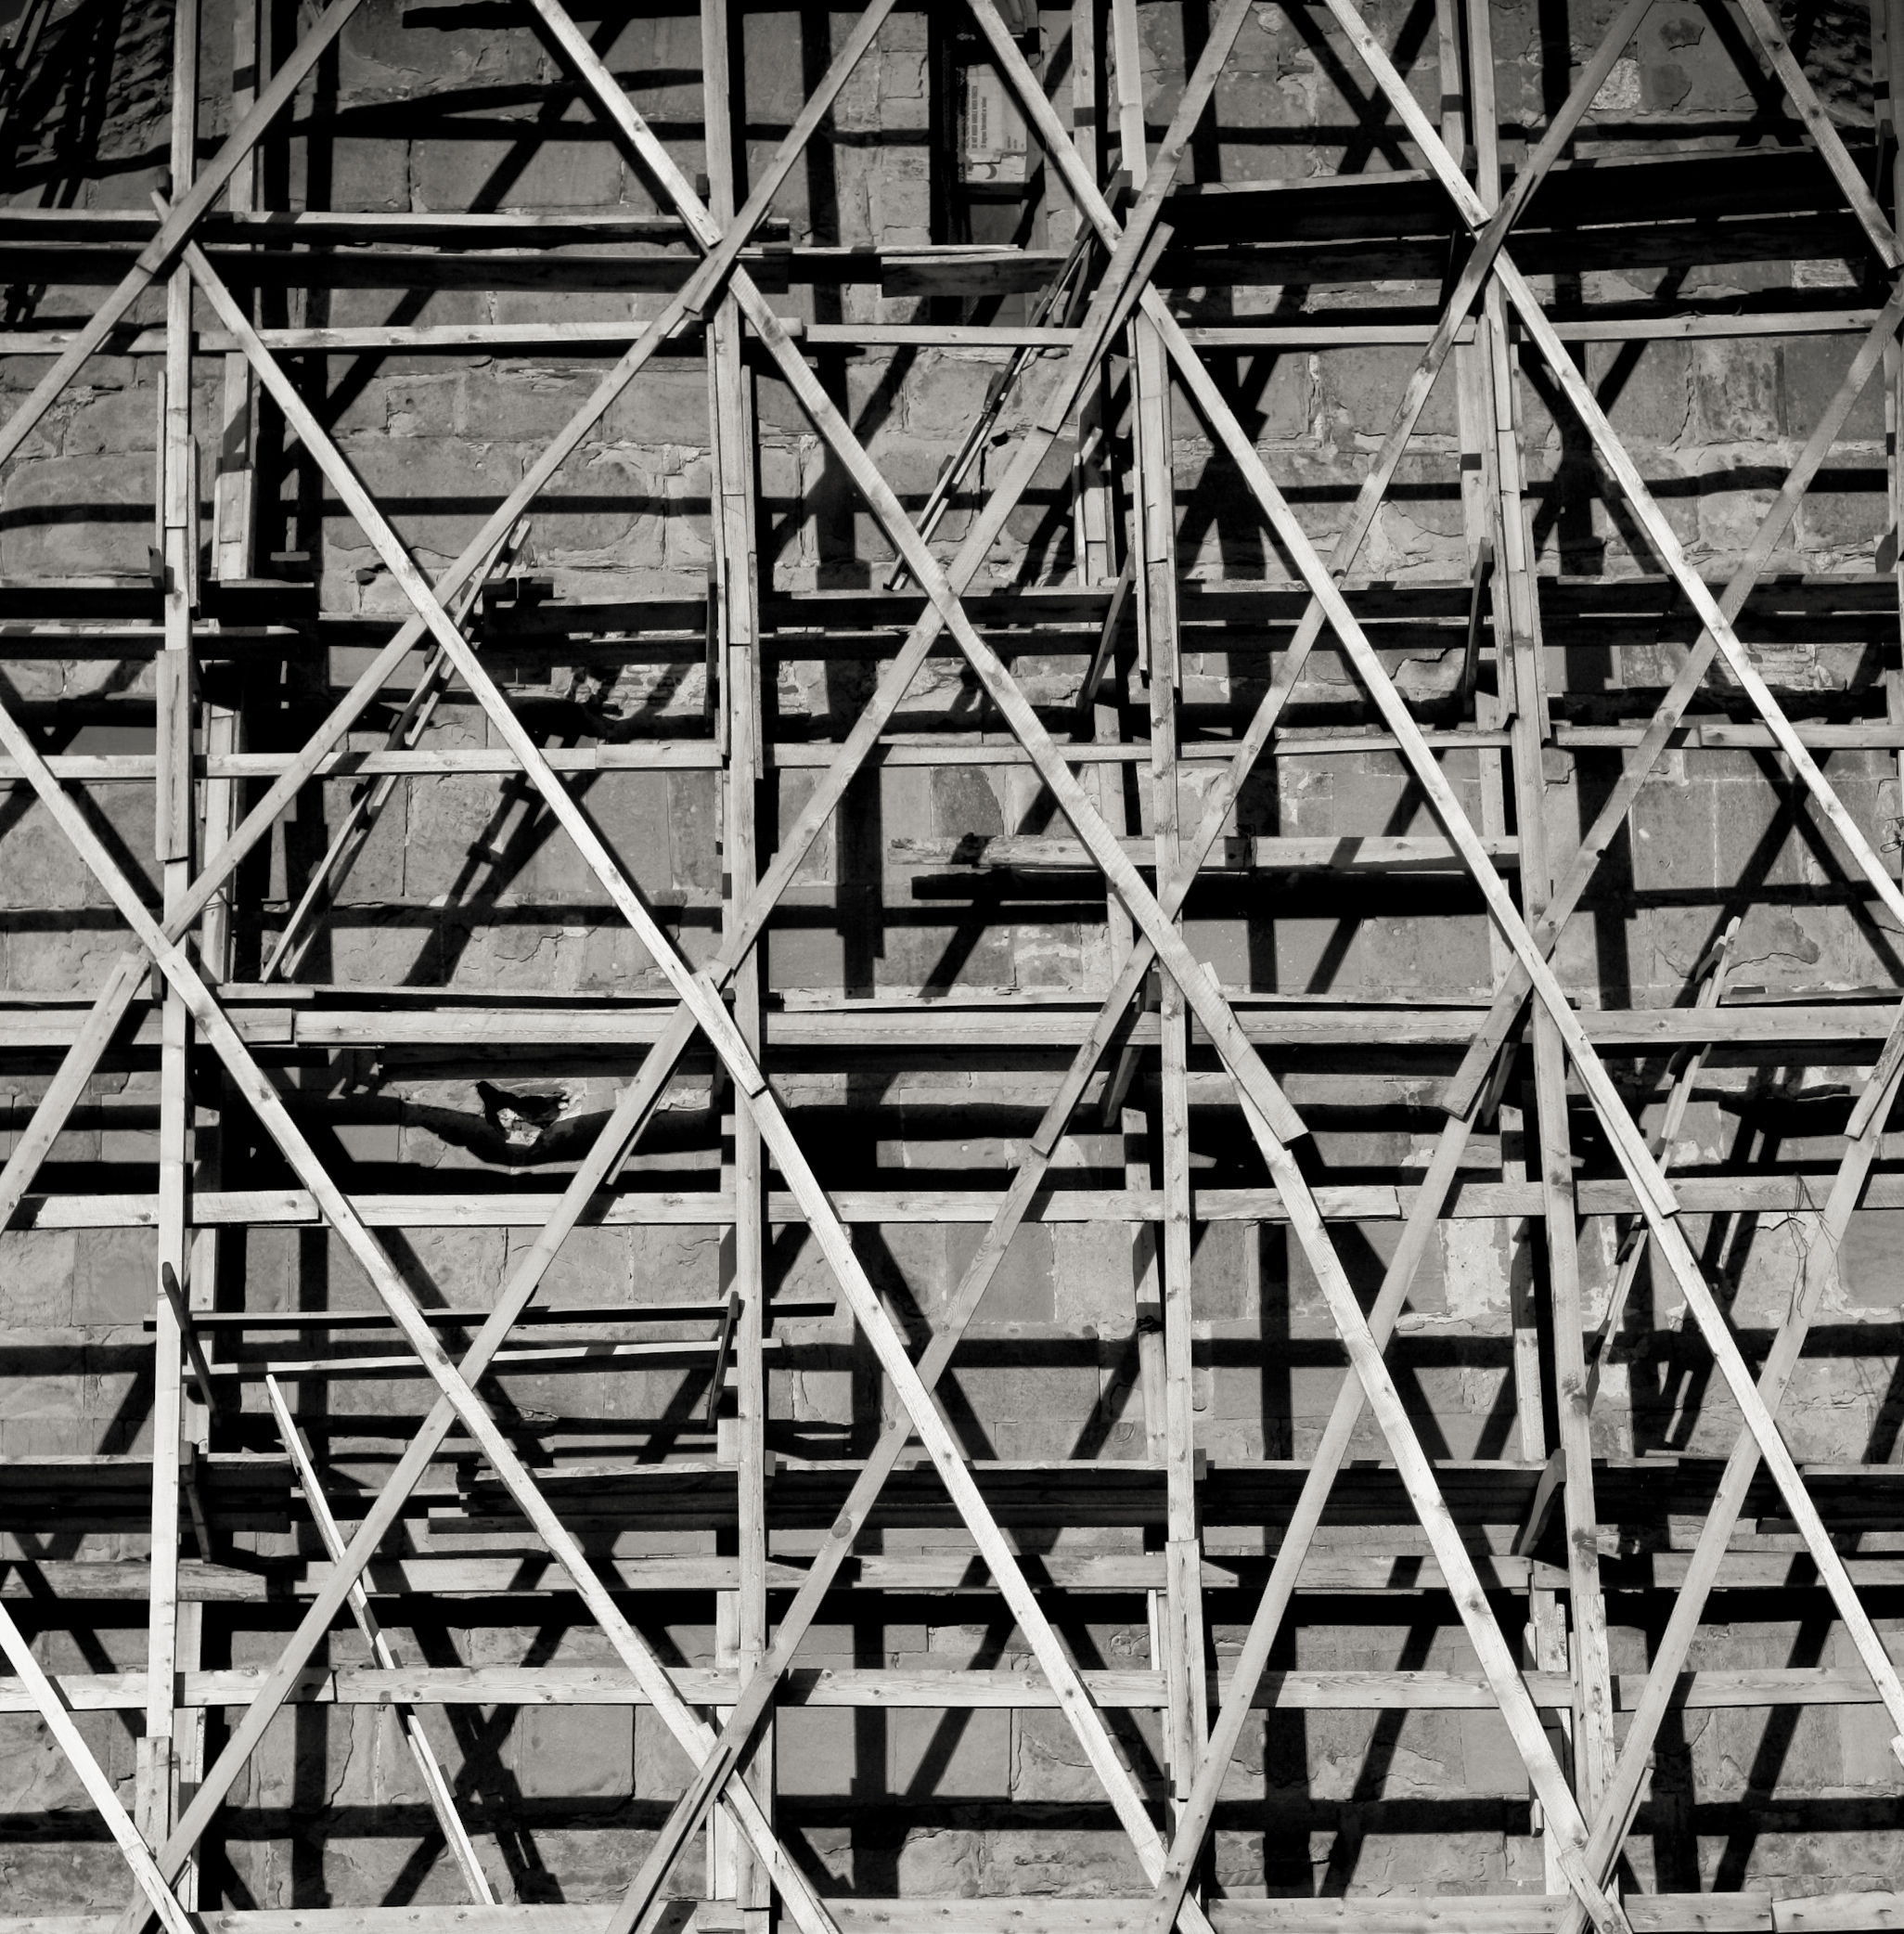
\includegraphics[width=0.95\textwidth]{\folder img/rhombus.jpg}
% \begin{center}
%   {\large ``In geometry, a rhombus or rhomb is a quadrilateral 
%     whose four sides all have the same length''}\par
%   Foto di pursanovd\par
%   \url{http://www.flickr.com/photos/pursanovd/3669422214/}\par
%   Licenza: Creative Commons Attribution 2.0\par
% \end{center}
% \newpage

\section{Generalità sui quadrilateri} 
  \label{sect:generalita_quadrilateri}

\subsection{Distanza di un punto da una retta e altezza di una 
  striscia di piano}

\begin{wrapfigure}{r}{0.3\textwidth}
  \centering% Copyright (c) 2015 Daniele Masini - d.masini.it@gmail.com

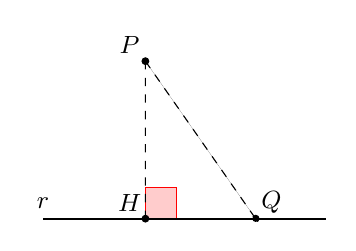
\begin{tikzpicture}[scale=1,font=\small]
\usetikzlibrary{calc}

\begin{scope}
\coordinate (r1) at (0.7,-2);
\coordinate (r2) at (4.3,-2);
\coordinate (s1) at (2,0.5);
\coordinate (s2) at (2,-2.5);
\coordinate (p) at (2,0);
\coordinate (h) at (intersection of r1--r2 and s1--s2);
\coordinate (q) at ($(r1)!0.75!(r2)$);

\draw[red, fill=red!20] (h) rectangle ([shift={(0.4,0.4)}]h);

\draw[thick] (r1) node[above] {$r$} -- (r2);
\draw[dashed] (p) -- (h);
\draw[fill] (p) circle (1.2pt) node [shift={(-.2,.2)}] {$P$};
\draw[fill] (h) circle (1.2pt) node [shift={(-.2,.2)}] {$H$};
\draw[fill,dashed] (p) -- (q) circle (1.2pt) node[shift={(.2,.2)}] {$Q$};

\end{scope}

\end{tikzpicture}

\end{wrapfigure}
Ricordiamo che come definizione di (\emph{misura} della) 
\emph{distanza di un punto da una retta} è stata presa la lunghezza 
del segmento congiungente il punto con il piede della perpendicolare 
mandata dal punto alla retta (vedi figura). Analogamente, per 
\emph{distanza tra due rette parallele}, detta anche \emph{altezza 
  della striscia di piano individuata dalle due rette parallele}, si 
intende la distanza di un punto qualsiasi di una retta dall'altra 
retta. Vogliamo far vedere ora che queste definizioni sono coerenti 
con il concetto di distanza tra due insiemi di punti come 
\emph{percorso più breve} che congiunge un qualsiasi punto del primo 
insieme con un generico punto appartenente al secondo insieme. Se 
congiungiamo, infatti, un generico punto $P$ sia con $H$, piede della 
perpendicolare alla retta $r$, che con un altro punto $Q\in r$, viene 
individuato un triangolo rettangolo $PHQ$, di cui $PH$ è un cateto e 
$PQ$ l'ipotenusa. Dal teorema sulle disuguaglianze degli elementi di 
un triangolo, l'ipotenusa è certamente maggiore di un cateto in 
quanto lato che si oppone ad angolo maggiore (quello retto). Dunque 
$PH$ è il segmento di lunghezza minore tra tutti quelli che 
congiungono $P$ con un punto della retta $r$.

\subsection{Generalità sui poligoni}

Se un poligono ha più di tre lati, allora può anche essere concavo. 
Ricordiamo che la somma degli angoli interni di un quadrilatero è 
$360\grado$.

\begin{definizione}
  Due lati non consecutivi di un quadrilatero si dicono \emph{opposti}; 
  analogamente sono detti \emph{opposti} due angoli non adiacenti allo 
  stesso lato.
\end{definizione}

Nella figura seguente sono rappresentati un quadrilatero concavo 
($Q_1$), un generico quadrilatero convesso ($Q_2$), un quadrilatero 
particolare a forma di ``aquilone'' ($Q_6$) e tre quadrilateri 
``notevoli'': $Q_3$ ha i lati opposti paralleli (a due a due), $Q_4$ 
e $Q_5$ hanno una coppia di lati opposti paralleli.


\begin{inaccessibleblock}[Figura: TODO]
  \begin{figure}[htb]
    \centering% Copyright (c) 2015 Daniele Masini - d.masini.it@gmail.com

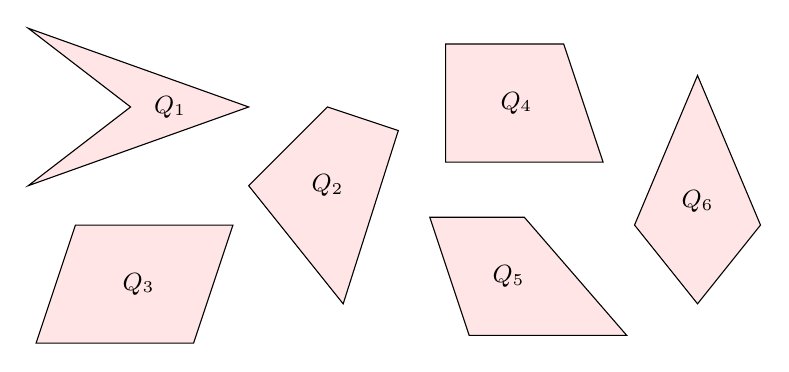
\begin{tikzpicture}[scale=1,font=\small]
\usetikzlibrary{calc}

\begin{scope}
\draw[fill=red!10] (0,0) -- (-1.3,1) -- (1.5,0) -- (-1.3,-1) -- cycle;
\node at (0.5,0) {$Q_1$};
\end{scope}

\begin{scope}[shift={(1.5cm,-1cm)}]
\draw[fill=red!10] (0,0) -- (1,1) -- (1.9,0.7) -- (1.2,-1.5) -- cycle;
\node at (1,0) {$Q_2$};
\end{scope}

\begin{scope}[shift={(-1.2cm,-3cm)}]
\draw[fill=red!10] (0,0) -- (0.5,1.5) -- (2.5,1.5) -- (2,0) -- cycle;
\node at (1.3,0.75) {$Q_3$};
\end{scope}

\begin{scope}[shift={(4cm,-.7cm)}]
\draw[fill=red!10] (0,0) -- (0,1.5) -- (1.5,1.5) -- (2,0) -- cycle;
\node at (0.9,0.75) {$Q_4$};
\end{scope}

\begin{scope}[shift={(4.3cm,-2.9cm)}]
\draw[fill=red!10] (0,0) -- (-0.5,1.5) -- (0.7,1.5) -- (2,0) -- cycle;
\node at (0.5,0.75) {$Q_5$};
\end{scope}

\begin{scope}[shift={(7.2cm,0cm)}]
\draw[fill=red!10] (0,0.4) -- (-0.8,-1.5) -- (0,-2.5) -- (0.8,-1.5) -- cycle;
\node at (0,-1.2) {$Q_6$};
\end{scope}

\end{tikzpicture}

  \end{figure}
\end{inaccessibleblock}

I quadrilateri che, come $Q_6$, hanno due lati consecutivi congruenti 
ed altri due lati consecutivi anch'essi congruenti, si dicono 
\emph{deltoidi}; i quadrilateri che, come $Q_3$, hanno i lati opposti 
paralleli si dicono \emph{parallelogrammi}; i quadrilateri che, come 
$Q_4$ e $Q_5$, hanno una coppia di lati opposti paralleli si dicono 
\emph{trapezi}.

\osservazione In analogia alla definizione di triangolo isoscele 
(come triangolo avente ``almeno'' due lati congruenti), alcuni autori 
definiscono trapezio un quadrilatero avente ``almeno'' una coppia di 
lati opposti paralleli: con questa definizione un parallelogramma è 
un particolare tipo di trapezio. Ricordiamo anche che Euclide, al 
contrario, classificava come trapezi tutti i quadrilateri che non 
fossero parallelogrammi. Noi useremo come definizione di 
\emph{trapezio} quella di un \emph{quadrilatero avente ``solo'' una 
  coppia di lati opposti paralleli}. Ci riferiremo al parallelogramma 
come a una figura piana costituita dall'intersezione di due strisce 
di piano non parallele fra loro; al trapezio come intersezione tra 
una striscia di piano ed un angolo convesso con vertice esterno alla 
striscia e lati che intersecano la striscia stessa. Poiché le strisce 
di piano sono convesse, sia i parallelogrammi sia i trapezi, come 
intersezioni di figure convesse, sono convessi.

\begin{procedura}
  Dato un segmento AB e un punto C, traccia un trapezio ABCD, con CD e AB lati 
paralleli:
  \begin{enumerate} [nosep]
    \item 
    Traccia il segmento AB, il punto C e il segmento BC.
    \item 
    Traccia la retta passante per C e parallela ad AB.
    \item 
    Traccia arbitrariamente un punto D su tale retta.
    \item  
    Costruisci il quadrilatero ABCD
  \end{enumerate}
\end{procedura}

\section{Trapezio e deltoide}
\label{sect:trapezio_deltoide}

Osserviamo le figure seguenti. I quadrilateri $ABCD$, $EFGH$, $IJKL$ 
e $MNOP$ sono trapezi perché hanno una coppia di lati opposti 
paralleli. Tali lati paralleli si dicono \emph{basi} e si distinguono 
in \emph{base maggiore} e \emph{base minore}. Gli altri lati si 
dicono \emph{lati obliqui}. La distanza tra le rette parallele si 
dice \emph{altezza} del trapezio.
Un trapezio avente i lati obliqui congruenti si dice \emph{isoscele}. 
Un trapezio avente un lato perpendicolare alle basi si dice 
\emph{rettangolo}. Un trapezio che non è né isoscele né rettangolo si 
dice \emph{scaleno}.


\begin{inaccessibleblock}[Figura: TODO]
  \begin{figure}[htb]
    \centering% Copyright (c) 2015 Daniele Masini - d.masini.it@gmail.com

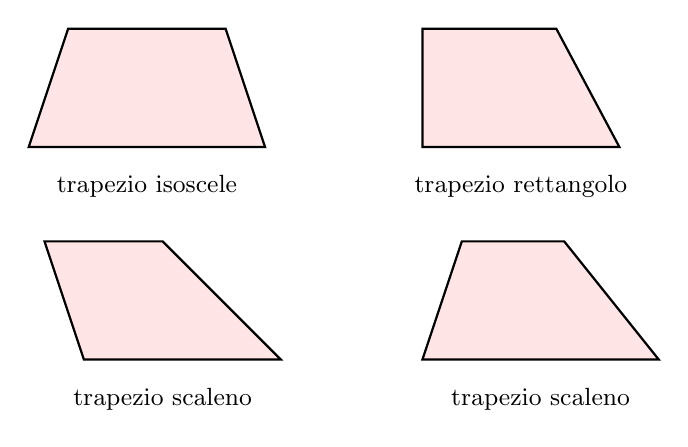
\begin{tikzpicture}[scale=1,font=\small]
\usetikzlibrary{calc}

\begin{scope}
\draw[thick, fill=red!10] (0,0) -- (2,0) -- (2.5,-1.5) -- (-0.5,-1.5) -- cycle;
\node at (1,-2) {trapezio isoscele};
\end{scope}

\begin{scope}[shift={(4.5cm,0cm)}]
\draw[thick, fill=red!10] (0,0) -- (1.7,0) -- (2.5,-1.5) -- (0,-1.5) -- cycle;
\node at (1.25,-2) {trapezio rettangolo};
\end{scope}

\begin{scope}[shift={(-0.3cm,-2.7cm)}]
\draw[thick, fill=red!10] (0,0) -- (1.5,0) -- (3,-1.5) -- (0.5,-1.5) -- cycle;
\node at (1.5,-2) {trapezio scaleno};
\end{scope}

\begin{scope}[shift={(5cm,-2.7cm)}]
\draw[thick, fill=red!10] (0,0) -- (1.3,0) -- (2.5,-1.5) -- (-0.5,-1.5) -- cycle;
\node at (1,-2) {trapezio scaleno};
\end{scope}

\end{tikzpicture}

  \end{figure}
\end{inaccessibleblock}

\subsection{Proprietà del trapezio}

In ogni trapezio, gli angoli adiacenti a ciascun lato obliquo sono 
supplementari. Essi, infatti, sono coniugati interni rispetto alle 
rette delle basi tagliate dalla trasversale individuata dal lato 
obliquo.

In un trapezio rettangolo, gli angoli adiacenti alla base maggiore 
sono uno retto ed uno acuto e gli angoli adiacenti alla base minore 
sono uno retto ed uno ottuso. Se un trapezio avesse quattro angoli 
retti, i lati obliqui sarebbero entrambi perpendicolari alle basi e 
di conseguenza paralleli tra loro. Dunque in questo caso il trapezio 
risulterebbe essere un parallelogramma.

Un trapezio scaleno può avere gli angoli adiacenti alla base maggiore 
entrambi acuti (e quindi gli angoli adiacenti alla base minore 
entrambi ottusi) oppure due angoli opposti entrambi acuti e gli altri 
ottusi (i due tipi di trapezio scaleno sono rappresentati nella 
figura precedente). I quattro angoli sono comunque non congruenti, 
altrimenti il trapezio risulterebbe isoscele nel primo caso e un 
parallelogramma nel secondo caso.

\begin{wrapfigure}{r}{0.3\textwidth}
  \centering% Copyright (c) 2015 Daniele Masini - d.masini.it@gmail.com

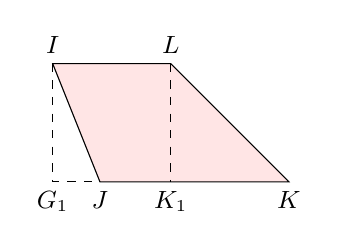
\begin{tikzpicture}[scale=1,font=\small]
\usetikzlibrary{calc}

\begin{scope}
\draw[fill=red!10] (0,0) coordinate (i) node[above] {$I$} -- (1.5,0) coordinate (l) node[above] {$L$} -- (3,-1.5) coordinate (k) node[below] {$K$} -- (0.6,-1.5) coordinate (j) node[below] {$J$} -- cycle;
\draw[dashed] (i) -- ($(j)!(i)!(k)$) coordinate (g1) node[below] {$G_1$} -- (j);
\draw[dashed] (l) -- ($(j)!(l)!(k)$) coordinate (k1) node[below] {$K_1$};
\end{scope}

\end{tikzpicture}

\end{wrapfigure}
In un trapezio isoscele, gli angoli adiacenti alla base maggiore sono 
acuti e quelli adiacenti alla base minore sono ottusi. 
A tal proposito, facciamo riferimento al trapezio $IJKL$ nella figura 
a fianco per dire che non può esistere un trapezio isoscele con due 
angoli acuti opposti e due angoli ottusi opposti. Infatti, se fosse 
$IJ\cong LK$, i triangoli $IG_1J$ e $LK_1K$ risulterebbero congruenti 
per il criterio particolare dei triangoli rettangoli, avendo 
congruenti le ipotenuse (i lati obliqui del trapezio $IJ$ e $LK$) ed 
una coppia di cateti (le altezze $IG_1$ e $LK_1$), da cui seguirebbe 
in particolare che $I\widehat{J}G_1\cong L\widehat{K}K_1$, e pertanto 
l'angolo in $K$ sarebbe supplementare dell'angolo in $J$, cosa che 
garantirebbe il parallelismo dei lati obliqui. Dunque, un ipotetico 
trapezio isoscele con due angoli acuti opposti sarebbe un 
parallelogramma.

\begin{wrapfigure}{r}{0.3\textwidth}
  \centering% Copyright (c) 2015 Daniele Masini - d.masini.it@gmail.com

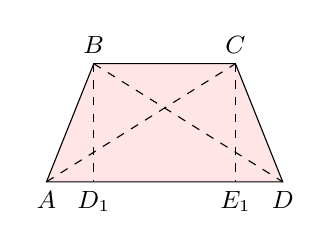
\begin{tikzpicture}[scale=1,font=\small]
\usetikzlibrary{calc}

\begin{scope}
\draw[fill=red!10] (0.1,0) coordinate (b) node[above] {$B$} -- (1.9,0) coordinate (c) node[above] {$C$} -- (2.5,-1.5) coordinate (d) node[below] {$D$} -- (-0.5,-1.5) coordinate (a) node[below] {$A$} -- cycle;
\draw[dashed] (b) -- ($(a)!(b)!(d)$) coordinate (d1) node[below] {$D_1$};
\draw[dashed] (c) -- ($(a)!(c)!(d)$) coordinate (e1) node[below] {$E_1$};
\draw[dashed] (b) -- (d);
\draw[dashed] (a) -- (c);
\end{scope}


\end{tikzpicture}

\end{wrapfigure}
Inoltre, se il trapezio è isoscele, gli angoli adiacenti a ciascuna 
delle basi sono congruenti. 
Infatti, in riferimento al trapezio $ABCD$, traccia le altezze $BD_1$ 
e $CE_1$ (tra loro congruenti perché entrambe rappresentano la 
distanza tra due rette parallele), i triangoli $AD_1B$ e $E_1DC$ 
risultano congruenti per il criterio particolare dei triangoli 
rettangoli, avendo congruenti le ipotenuse (i lati obliqui del 
trapezio) ed una coppia di cateti (le altezze del trapezio). Pertanto 
i rimanenti elementi risultano ordinatamente congruenti: 
$B\widehat{A}D\cong A\widehat{D}C$, $A\widehat{B}D_1\cong 
D\widehat{C}E_1$, $AD_1\cong E_1D$.

Dunque sono congruenti  anche le proiezioni dei lati obliqui sulla 
base maggiore. 
Quindi anche $A\widehat{B}C\cong B\widehat{C}D$ in quanto somme di 
angoli congruenti $A\widehat{B}D_1+\widehat{R}\cong 
D\widehat{C}E_1+\widehat{R}$.

In un trapezio isoscele, inoltre, anche le due diagonali sono 
congruenti. Infatti, in riferimento sempre al trapezio $ABCD$ in 
figura, i triangoli $ABC$ e $DCB$ risultano congruenti per il primo 
criterio, avendo $BC$ in comune, $AB\cong CD$ per ipotesi e gli 
angoli compresi (adiacenti alla base minore) congruenti per quanto 
appena dimostrato. Di conseguenza, i rimanenti elementi sono 
ordinatamente congruenti, in particolare i terzi lati (che sono, 
appunto, le diagonali $AC$ e $BD$ del trapezio).

\newpage %---------------------------------------------------

\subsection{Proprietà del deltoide}

\begin{wrapfigure}{l}{0.3\textwidth}
  \centering% Copyright (c) 2015 Daniele Masini - d.masini.it@gmail.com

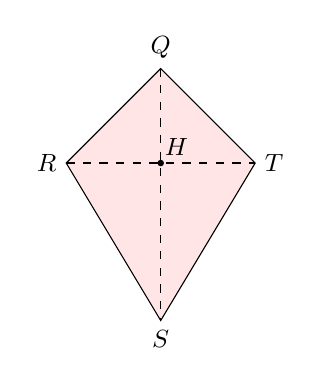
\begin{tikzpicture}[scale=0.8,font=\small]
\usetikzlibrary{calc}

\begin{scope}
\draw[fill=red!10] (0,0) coordinate (q) node[above] {$Q$} -- (1.5,-1.5) coordinate (t) node[right] {$T$} -- (0,-4) coordinate (s) node[below] {$S$} -- (-1.5,-1.5) coordinate (r) node[left] {$R$} -- cycle;
\coordinate (h) at (intersection of r--t and q--s);
\draw[dashed] (q) -- (s);
\draw[dashed] (r) -- (t);
\draw[fill] (h) circle (1.2pt) node[shift={(0.2,0.2)}] {$H$};
\end{scope}


\end{tikzpicture}

\end{wrapfigure}

Il poligono $QRST$ nella figura a fianco è un deltoide, ha i lati a 
due a due congruenti $QR\cong QT$ e $RS\cong TS$. Tracciamo le 
diagonali $QS$ ed $RT$. I triangoli $QRT$ e $STR$ sono isosceli sulla 
base comune $RT$. Dunque, se chiamiamo $H$ il punto medio di $RT$, 
$QH$ ed $SH$ sono mediane, bisettrici e altezze (relative alla base 
ed agli angoli al vertice dei due triangoli isosceli), per cui $QS$ è 
perpendicolare ad $RT$ e passa per il punto $H$. Quindi le due 
diagonali sono perpendicolari e si incontrano nel punto medio di 
$RT$. Inoltre i triangoli $SQR$ ed $STQ$ sono congruenti per il terzo 
criterio, pertanto $Q\widehat{R}S\cong Q\widehat{T}S$.

I quattro lati di un deltoide non potrebbero essere tutti congruenti, 
in quanto, dalla congruenza degli angoli opposti banalmente 
deducibile, risulterebbero i lati opposti paralleli, e quindi il 
deltoide sarebbe un parallelogramma. Non è al contrario escluso che 
un angolo possa essere retto (ma non più di uno, altrimenti il 
deltoide sarebbe un parallelogramma), mentre gli angoli ottusi possono 
essere uno, due o tre (come pure gli angoli acuti).

Lasciamo al lettore il compito di provare queste semplici proprietà, 
costruendo vari tipi di deltoidi.

\begin{procedura}
  Costruisci un trapezio isoscele, cioè con due lati congruenti:
  \begin{enumerate} [nosep]
    \item 
    Traccia il segmento AB, il punto C e il segmento BC.
    \item 
    Traccia la retta r passante per C e parallela ad AB.
    \item 
    Traccia la circonferenza di centro A e raggio BC.    
    \item 
    Chiama D e E le due intersezioni della retta r con la circonferenza ( in 
modo che risulti CD<CE )  
    \item 
    ABCD è il trapezio isoscele.    
    \item 
    ABCE invece un parallelogramma... un trapezio particolare!
    La suddetta costruzione quindi oltre a permetterti di disegnare un trapezio 
isoscele, ti consente di costruire un parallelogramma, che ha come lati due 
segmenti consecutivi dati.
  \end{enumerate}
\end{procedura}

\section{Proprietà dei parallelogrammi}
  \label{sect:proprieta_parallelogrammi}

Ricordiamo che, per definizione, un parallelogramma è un quadrilatero 
che ha i lati opposti paralleli.

\begin{teorema}
  In ogni parallelogramma:
  \begin{enumerate*}
    \item gli angoli adiacenti allo stesso lato (a ciascun lato) sono 
    supplementari;
    \item gli angoli opposti sono congruenti;
    \item ciascuna diagonale divide il parallelogramma in due triangoli 
    congruenti;
    \item i lati opposti sono congruenti;
    \item le diagonali si dividono scambievolmente per metà. 
  \end{enumerate*}
\end{teorema}

\noindent Ipotesi: $AB\parallel CD$, $AD\parallel BC$.


\begin{inaccessibleblock}[Figura: TODO]
  \begin{figure}[htb]
    \centering% Copyright (c) 2015 Daniele Masini - d.masini.it@gmail.com

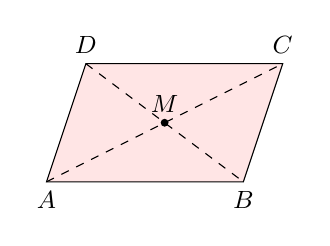
\begin{tikzpicture}[scale=1,font=\small]
\usetikzlibrary{calc}

\begin{scope}
\draw[fill=red!10] (0,0) coordinate (a) node[below] {$A$} -- (2.5,0) coordinate (b) node[below] {$B$} -- (3,1.5) coordinate (c) node[above] {$C$} -- (0.5,1.5) coordinate (d) node[above] {$D$} -- cycle;
\coordinate (m) at (intersection of d--b and a--c);
\draw[dashed] (a) -- (c);
\draw[dashed] (d) -- (b);
\draw[fill] (m) circle (1.2pt) node[above] {$M$};
\end{scope}


\end{tikzpicture}

  \end{figure}
\end{inaccessibleblock}

\begin{proof}~\\
  \begin{enumerate*}
    
    \item Tesi: $D\widehat{A}B+A\widehat{B}C\cong\pi$, 
    $A\widehat{B}C+B\widehat{C}D\cong\pi$, 
    $B\widehat{C}D+C\widehat{D}A\cong\pi$ ($\pi$ è l'angolo piatto).\\
    Se $AB\parallel CD$, gli angoli in $A$ e $D$ sono supplementari, e 
    così pure gli angoli in $B$ e $C$, in quanto coniugati interni 
    rispetto alle due rette parallele tagliate rispettivamente dalle 
    trasversali $AD$ e $BC$. Analogamente, se $AD\parallel BC$, gli 
    angoli in $A$ e $B$ sono supplementari, ed anche gli angoli in $C$ e 
    $D$. La tesi 1 è pertanto dimostrata.
    
    \item Tesi: $A\widehat{B}C\cong C\widehat{D}A$, $D\widehat{A}B\cong 
    B\widehat{C}D$.\\
    Dunque, se è vera l'ipotesi, possiamo considerare verificate le 
    congruenze della tesi 1. Da queste segue che gli angoli opposti sono 
    congruenti in quanto supplementari dello stesso angolo: gli angoli in 
    $A$ e $C$ sono supplementari entrambi dell'angolo in $B$, gli angoli 
    in $B$ e in $D$ sono entrambi supplementari dell'angolo in $A$. La 
    tesi 2 è pertanto dimostrata.
    
    \item Tesi: $ABC\cong CDA$, $DAB\cong BCD$.\\
    Tracciamo ora una diagonale, ad esempio $AC$, e consideriamo i due 
    triangoli che si vengono a formare, $ABC$ e $ACD$. Essendo 
    $AB\parallel CD$, risulta $D\widehat{C}A\cong C\widehat{A}B$ ed 
    essendo $AD\parallel BC$, risulta $D\widehat{A}C\cong A\widehat{C}B$, 
    in quanto sono coppie di angoli alterni interni, i primi rispetto 
    alle rette $AB$ e $CD$ tagliate dalla trasversale $AC$, gli altri 
    rispetto alle rette parallele $AD$ e $BC$ tagliate dalla trasversale 
    $AC$. I due triangoli dunque, avendo in comune il lato $AC$, 
    risultano congruenti per il secondo criterio. Analogamente, applicando 
    il ragionamento precedente ai triangoli $ABD$ e $DBC$ dopo aver 
    tracciato la diagonale $DB$, concludiamo che anche i due triangoli 
    $ADB$ e $DBC$ risultano congruenti per il secondo criterio. Pertanto 
    la tesi 3 è dimostrata.
    
    \item Tesi: $AB\cong CD$, $AD\cong BC$.\\
    Dunque, se è vera l'ipotesi, possiamo considerare verificate le 
    congruenze della tesi 3. Dalla congruenza dei triangoli $ABC$ e $CDA$ 
    segue la congruenza dei lati $AB$ e $CD$, dalla congruenza dei 
    triangoli $DAB$ e $BCD$ segue la congruenza dei lati $AD$ e $BC$. 
    Pertanto la tesi 4 è dimostrata.
    
    \item Tesi: $AM\cong MC$, $DM\cong MB$.\\
    Dopo aver tracciato entrambe le diagonali, chiamiamo $M$ il loro 
    punto di intersezione. Confrontiamo i triangoli $ABM$ e $CDM$: essi 
    risultano congruenti per il secondo criterio, in quanto $AB\cong CD$ 
    (tesi 4), $D\widehat{A}C\cong A\widehat{C}B$ e $D\widehat{C}A\cong 
    C\widehat{A}B$ (come visto nel punto 3 della dimostrazione). Quindi 
    anche i rimanenti elementi risultano ordinatamente congruenti, in 
    particolare $AM\cong MC$ e $DM\cong MB$. Pertanto anche la tesi 5 è 
    dimostrata.
  \end{enumerate*}
\end{proof}

Il teorema precedente è invertibile. Precisamente vale il teorema 
seguente:
\begin{teorema}
  Se in un quadrilatero è verificata una delle seguenti ipotesi:
  \begin{enumerate*}
    \item gli angoli adiacenti allo stesso lato (a ciascun lato) sono 
    supplementari;
    \item gli angoli opposti sono congruenti;
    \item ciascuna diagonale divide il quadrilatero in due triangoli 
    congruenti;
    \item i lati opposti sono congruenti;
    \item le diagonali si dividono scambievolmente per metà;
    \item due lati opposti sono paralleli e congruenti;
  \end{enumerate*}
  allora il quadrilatero è un parallelogramma.
\end{teorema}


\begin{inaccessibleblock}[Figura: TODO]
  \begin{figure}[htb]
    \centering% Copyright (c) 2015 Daniele Masini - d.masini.it@gmail.com

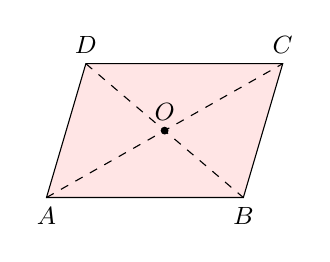
\begin{tikzpicture}[scale=1,font=\small]
\usetikzlibrary{calc}

\begin{scope}
\draw[fill=red!10] (0,0) coordinate (a) node[below] {$A$} -- (2.5,0) coordinate (b) node[below] {$B$} -- (3,1.7) coordinate (c) node[above] {$C$} -- (0.5,1.7) coordinate (d) node[above] {$D$} -- cycle;
\coordinate (o) at (intersection of d--b and a--c);
\draw[dashed] (a) -- (c);
\draw[dashed] (d) -- (b);
\draw[fill] (o) circle (1.2pt) node[above] {$O$};
%\node at (1.5,-1) {(a)};
\end{scope}

%\begin{scope}[xshift=5cm]
%\draw[fill=red!10] (0,0) coordinate (e) node[below] {$E$} -- (2.5,0) coordinate (f) node[below] {$F$} -- (3,1.7) coordinate (g) node[above] {$G$} -- (0.5,1.7) coordinate (h) node[above] {$H$} -- cycle;
%\coordinate (o) at (intersection of d--b and a--c);
%\draw[dashed] (e) -- (g);
%\draw[dashed] (f) -- (h);
%\draw[fill] (o) circle (1.2pt) node[left] {$O$};
%\node at (1.5,-1) {(b)};
%\end{scope}


\end{tikzpicture}

  \end{figure}
\end{inaccessibleblock}

\begin{proof}~\\
  \begin{enumerate*}
    \item Sia per ipotesi $D\widehat{A}B+A\widehat{B}C\cong \pi$ (dove 
    $\pi$ è l'angolo piatto). Tali angoli, rispetto alle rette $AD$ ed 
    $BC$ tagliate dalla trasversale $AB$ sono coniugati interni, allora 
    per quanto visto nel capitolo precedente sul parallelismo, le rette 
    $AD$ e $BC$ sono parallele perché formano angoli coniugati interni 
    supplementari con la trasversale $AB$. Analogamente, se 
    $A\widehat{B}C+B\widehat{C}D\cong \pi$, le rette $AB$ ed $DC$ sono 
    parallele. Dunque $ABCD$ è un parallelogramma, avendo i lati opposti 
    paralleli.
    \item Poiché la somma degli angoli interni di un quadrilatero misura 
    $360\grado$, se gli angoli opposti sono congruenti, vuol dire che 
    $D\widehat{A}B+A\widehat{B}C+B\widehat{C}D+C\widehat{D}A\cong 
    2D\widehat{A}B+2A\widehat{B}C\cong 2\pi$, per cui 
    $D\widehat{A}B+A\widehat{B}C\cong\pi$, cioè gli angoli adiacenti allo 
    stesso lato sono supplementari e per la dimostrazione precedente 
    $ABCD$ è un parallelogramma.
    \item Essendo i triangoli $ABC$ e $BDC$ congruenti, l'angolo 
    $A\widehat{B}D$ risulta congruente all'angolo $B\widehat{D}C$ ed 
    essendo questi angoli alterni interni rispetto alle rette $AB$ e $CD$ 
    tagliate dalla trasversale $BD$ allora le due rette $AB$ e $CD$ 
    saranno parallele. In maniera analoga $A\widehat{D}B\cong 
    D\widehat{B}C$ e quindi, essendo alterni interni rispetto alle rette 
    $BC$ e $AD$ intersecate dalla trasversale $BD$ si ha che anche 
    $BC\parallel AD$. Quindi $ABCD$ è un parallelogramma.
    %\item Sia $FH$ una diagonale del quadrilatero $EFGH$, figura (b), 
    allora i vertici $E$ e $G$ cadranno su semipiani opposti rispetto 
    alla retta $FH$. Nel caso in cui i due triangoli $FHE$ e $FHG$, oltre 
    che congruenti, sono isosceli sulla base $FH$, il quadrilatero $EFGH$ 
    ha gli angoli opposti congruenti, per cui è un parallelogramma per la 
    tesi 2. Se, al contrario, $FHE$ e $FHG$ non sono isosceli sulla base 
    $FH$, allora dobbiamo considerare due sottocasi distinti, evidenziati 
    in figura, con quattro diversi quadrilateri. Se fosse $EH\cong HG$ e 
    $EF\cong FG$, la figura risulterebbe un deltoide e l'altra diagonale 
    $EG$ non dividerebbe il quadrilatero in due triangoli congruenti. 
    Rimane l'altro sottocaso possibile, $EF\cong HG$ e $EH\cong FG$, ed 
    inoltre $A\widehat{D}B\cong D\widehat{B}C$, $A\widehat{B}D\cong 
    B\widehat{D}C$ e $D\widehat{A}B\cong B\widehat{C}D$, pertanto il 
    quadrilatero risulta essere un parallelogramma per la 2. Dunque in 
    ogni caso possibile la tesi è dimostrata.
    \item Consideriamo la diagonale $AC$. Il quadrilatero $ABCD$ è diviso 
    in due triangoli $ABC$ e $ACD$ congruenti per il terzo criterio. 
    Pertanto $A\widehat{C}D\cong C\widehat{A}B$ e $A\widehat{C}B\cong 
    C\widehat{A}D$, coppie di angoli alterni interni, nell'ordine 
    rispetto alle rette $AB$ e $CD$ e rispetto alle rette $AD$ ed $BC$, 
    tagliate dalla trasversale $AC$. Dunque i lati opposti del 
    quadrilatero $ABCD$ risultano paralleli, cioè è un parallelogramma.
    \item Detto $O$ il punto di incontro delle diagonali, i triangoli 
    $OAB$ ed $OCD$ risultano congruenti per il primo criterio, in quanto 
    $OA\cong OC$, $OD\cong OB$ e gli angoli tra essi compresi sono 
    congruenti perché opposti al vertice. Di conseguenza, risulta anche 
    $D\widehat{C}A\cong C\widehat{A}B$, che sono angoli alterni interni 
    rispetto alle rette $DC$ ed $AB$ tagliate dalla trasversale $AC$, 
    pertanto $DC\parallel AB$. Analogamente, considerando i triangoli 
    congruenti $OBC$ ed $ODA$ si ha anche $BC\parallel AD$. Dunque $ABCD$ 
    è un parallelogramma.
    \item Supponiamo $AB$ e $CD$ paralleli e congruenti. Tracciata la 
    diagonale $AC$, risulta $D\widehat{C}A\cong C\widehat{A}B$ e dunque i 
    triangoli $ACD$ e $CAB$ risultano congruenti per il primo criterio. 
    Di conseguenza risulta $AD\cong BC$, per cui il quadrilatero ha anche 
    l'altra coppia di lati opposti congruenti. $ABCD$ è dunque un 
    parallelogramma per la 4.
  \end{enumerate*}
\end{proof}


\begin{procedura}
  Costruire un parallelogramma dai tre suoi vertici:
  \begin{enumerate} [nosep]
    \item 
    Siano A, B, C tre punti del piano, ordinati in senso antiorario.
    \item 
    Traccia il segmento AC.
    \item 
    Costruisci il punto medio del segmento AC e denominalo M.
    \item 
    Traccia la semiretta di origine B passante per M.
    \item 
    Tracci­a la circonferenza di centro M e raggio MB.
    \item 
    Denomina D il punto,  diverso da B, di intersezione della semiretta con la 
circonferenza.
    \item 
    Il quadrilatero ABCD è il parallelogramma che soddisfa alle richieste
  \end{enumerate}
\end{procedura}


\begin{procedura}
  Costruisci un quadrilatero convesso ABCD con le coppie di lati opposti 
congruenti.(AB congruente a DC e AD congruente a BC):
  \begin{enumerate} [nosep]
    \item 
    Traccia un punto A e una semiretta di origine A.
    \item 
    Considera un segmento AB, con B appartenente a tale semiretta, e 
l'ulteriore segmento BC, con C non appartenente alla semiretta.
    \item 
    Traccia la circonferenza di centro C e raggio congruente ad AB.
    \item 
    Traccia la circonferenza di centro A e raggio BC.
    
    \item
    Il punto D è, dei due punti di intersezione fra le due circonferenze, 
quello che appartiene al semipiano originato dalla retta AB contenente C.
    \item 
    Il qadrilatero ABCD è un parallelogramma.
\end{enumerate}
\end{procedura}

\section{Parallelogrammi particolari}
  \label{sect:parallelogrammi_particolari}

I parallelogrammi possono essere sia equiangoli sia equilateri.

\noindent\begin{minipage}{0.7\textwidth}\parindent15pt
  Se un parallelogramma è equiangolo, dato che la somma degli angoli 
  interni è $360\grado$, deve avere quattro angoli retti: questo 
  succede quando due lati opposti, paralleli tra loro, sono 
  perpendicolari all’altra coppia di lati opposti. Un tale 
  parallelogramma si chiama \emph{rettangolo}.
  
  Se un parallelogramma è equilatero, vuol dire che ciascuna diagonale 
  lo divide in due triangoli isosceli. Un tale parallelogramma si 
  chiama \emph{rombo}.
  
  Un parallelogramma sia equiangolo sia equilatero deve essere 
  contemporaneamente un rettangolo ed un rombo: l'unico tipo di 
  quadrilatero regolare, il \emph{quadrato}. Infatti un quadrilatero, 
  per essere regolare, deve necessariamente avere quattro angoli retti; 
  è quindi un parallelogramma, prima ancora che un rettangolo, perché 
  due angoli retti, oltre ad essere congruenti, sono anche 
  supplementari; inoltre è un rombo in quanto è un parallelogramma con 
  quattro lati congruenti.
\end{minipage}\hfil
\begin{minipage}{0.3\textwidth}
  \centering% Copyright (c) 2015 Daniele Masini - d.masini.it@gmail.com

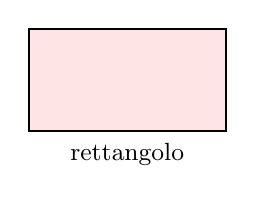
\begin{tikzpicture}[scale=1,font=\small]
\usetikzlibrary{calc}

\begin{scope}
\draw[thick, fill=red!10] (0,0) coordinate (a) -- (2.5,0) coordinate (b) -- (2.5,1.3) coordinate (c) -- (0,1.3) coordinate (d) -- cycle;
\node at (1.25,-0.3) {rettangolo};
\end{scope}

\end{tikzpicture}
\\~\\
  \centering% Copyright (c) 2015 Daniele Masini - d.masini.it@gmail.com

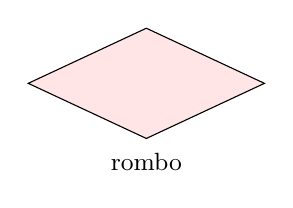
\begin{tikzpicture}[scale=1,font=\small]
\usetikzlibrary{calc}

\begin{scope}
\draw[fill=red!10] (0,0) coordinate (a) -- (1.5,-0.7) coordinate (b) -- (3,0) coordinate (c) -- (1.5,0.7) coordinate (d) -- cycle;
\node at (1.5,-1) {rombo};
\end{scope}

\end{tikzpicture}
\\~\\
  \centering% Copyright (c) 2015 Daniele Masini - d.masini.it@gmail.com

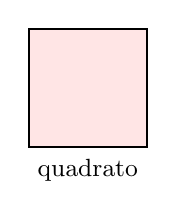
\begin{tikzpicture}[scale=1,font=\small]
\usetikzlibrary{calc}

\begin{scope}
\draw[thick, fill=red!10] (0,0) coordinate (a) -- (1.5,0) coordinate (b) -- (1.5,1.5) coordinate (c) -- (0,1.5) coordinate (d) -- cycle;
\node at (0.75,-0.3) {quadrato};
\end{scope}

\end{tikzpicture}

\end{minipage}

A parte le proprietà particolari insite nelle stesse definizioni, il 
rettangolo e il rombo si distinguono tra loro e dagli altri 
parallelogrammi per alcune proprietà riguardanti le diagonali. 
Naturalmente il quadrato gode delle proprietà sia del rettangolo sia 
del rombo.
Ricordiamo che in un parallelogramma le diagonali si dividono 
scambievolmente per metà. Ora mostreremo che in un rettangolo le 
diagonali sono congruenti ed in un rombo sono perpendicolari.

\begin{teorema}
  In ogni rettangolo le diagonali sono congruenti. Viceversa, se un 
  parallelogramma ha le diagonali congruenti, allora è un rettangolo.
\end{teorema}


\begin{inaccessibleblock}[Figura: TODO]
  \begin{figure}[htb]
    \centering% Copyright (c) 2015 Daniele Masini - d.masini.it@gmail.com

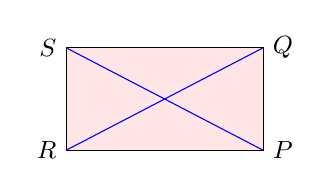
\begin{tikzpicture}[scale=1,font=\small]
\usetikzlibrary{calc}

\begin{scope}
\draw[fill=red!10] (0,0) coordinate (a) node[left] {$R$} -- (2.5,0) coordinate (b) node[right] {$P$} -- (2.5,1.3) coordinate (c) node[right] {$Q$} -- (0,1.3) coordinate (d) node[left] {$S$} -- cycle;
\draw[blue] (a) -- (c);
\draw[blue] (b) -- (d);
\end{scope}

\end{tikzpicture}

  \end{figure}
\end{inaccessibleblock}

\begin{proof}
  Sia $RPQS$ un rettangolo; tracciate le diagonali $RQ$ e $PS$, 
  confrontiamo i triangoli $SRP$ e $RPQ$. Tali triangoli rettangoli 
  hanno il cateto $RP$ in comune ed hanno gli altri cateti, $SR$ e 
  $PQ$, rispettivamente congruenti in quanto lati opposti di un 
  rettangolo. Dunque $SRP$ e $RPQ$ sono congruenti per il primo criterio 
  e di conseguenza devono avere congruenti anche le ipotenuse $SP$ e 
  $RQ$, le quali sono le diagonali del rettangolo.
  
  Sia $RPQS$ un parallelogramma avente le diagonali $RQ$ e $PS$ 
  congruenti, sempre confrontando i triangoli $SRP$ e $RPQ$, possiamo 
  affermare che tali triangoli sono congruenti per il terzo criterio, 
  perché hanno il lato $RP$ in comune, i lati $RS$ e $QP$ congruenti in 
  quanto lati opposti di un parallelogramma ed i lati $SP$ e $RQ$ 
  congruenti per ipotesi. Dunque anche gli angoli devono essere 
  ordinatamente congruenti, in particolare  perché opposti ai lati 
  congruenti $SP$ e $RQ$. Ma tali angoli sono anche supplementari in 
  quanto adiacenti allo stesso lato $RP$ di un parallelogramma e 
  pertanto devono risultare retti. Dunque il quadrilatero $RPSQ$ è un 
  rettangolo.
\end{proof}

\begin{teorema}
  In ogni rombo le diagonali sono perpendicolari e sono anche 
  bisettrici degli angoli aventi per vertici i loro estremi. Viceversa, 
  se un parallelogramma ha le diagonali perpendicolari è un rombo; 
  inoltre, se un angolo di un parallelogramma è diviso a metà dalla 
  diagonale passante per il suo vertice, allora il parallelogramma è un 
  rombo.
\end{teorema}


\begin{inaccessibleblock}[Figura: TODO]
  \begin{figure}[htb]
    \centering% Copyright (c) 2015 Daniele Masini - d.masini.it@gmail.com

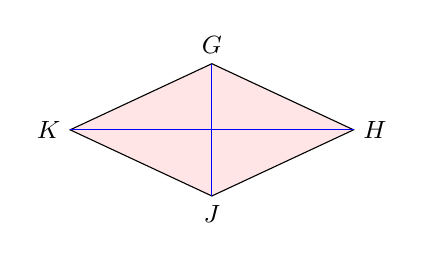
\begin{tikzpicture}[scale=1.2,font=\small]
\usetikzlibrary{calc}

\begin{scope}
\draw[fill=red!10] (0,0) coordinate (a) node[left] {$K$} -- (1.5,-0.7) coordinate (b) node[below] {$J$} -- (3,0) coordinate (c) node[right] {$H$} -- (1.5,0.7) coordinate (d) node[above] {$G$} -- cycle;
\draw[blue] (a) -- (c);
\draw[blue] (b) -- (d);
\end{scope}

\end{tikzpicture}

  \end{figure}
\end{inaccessibleblock}

\begin{proof}
  Notiamo che, in ciascuna delle fasi della dimostrazione, è tra le 
  ipotesi del teorema che $JHGK$ sia un parallelogramma. Ricordiamo che 
  le diagonali di $JHGK$ vengono divise a metà dal loro punto di 
  intersezione, che chiamiamo $M$, per cui risulta $JM\cong MG$ e 
  $HM\cong MK$.
  \begin{enumeratea}
    \item Se supponiamo che $JHGK$ sia un rombo, i triangoli $JHG$, 
    $HGK$, $GKJ$ e $KJH$ risultano isosceli, per cui le mediane $HM$, 
    $GM$, $KM$ e $JM$ sono anche altezze e bisettrici, per cui la prima 
    parte del teorema è dimostrata.
    \item Se supponiamo che $JG$ e $HK$ siano perpendicolari, in 
    particolare i triangoli rettangoli $JHM$, $HGM$, $GKM$ e $KJM$ 
    risultano congruenti per il primo criterio, avendo congruenti i 
    cateti. Dunque risultano congruenti anche le ipotenuse, che sono i 
    lati del parallelogramma $JHGK$, il quale pertanto risulta essere un 
    rombo.
    \item Se supponiamo ad esempio $K\widehat{G}J\cong J\widehat{G}H$, 
    essendo anche $K\widehat{G}J\cong G\widehat{J}H$ in quanto alterni 
    interni rispetto alle rette parallele $KG$ e $JH$ tagliate dalla 
    trasversale $GJ$, dalla proprietà transitiva della congruenza segue 
    che $G\widehat{J}H\cong J\widehat{G}H$, per cui il triangolo $JGH$ 
    risulta isoscele sulla base $JG$. Dunque il parallelogramma $JHGK$ ha 
    due lati consecutivi congruenti, e quindi i quattro lati congruenti, 
    ed è pertanto un rombo.
  \end{enumeratea}
\end{proof}

I teoremi precedenti si estendono automaticamente ai quadrati.
\begin{corollario}
  Le diagonali di un quadrato sono fra loro congruenti e perpendicolari 
  e dividono per metà gli angoli. Viceversa, se un parallelogramma ha 
  le diagonali congruenti e perpendicolari, allora è un quadrato; 
  inoltre, se le diagonali di un parallelogramma sono congruenti ed un 
  angolo è diviso a metà da una diagonale, allora il parallelogramma è 
  un quadrato.
\end{corollario}

\begin{procedura}
  Dato un segmento AB, costruisci un rombo di lato AB:
  \begin{enumerate} [nosep]
    \item 
    Traccia il segmento AB. 
    \item 
    Traccia la circonferenza con il centro in B passante per A.
    \item 
    Traccia un quasiasi punto appartenente alla circonferenza: denominalo C.
    \item 
    Traccia la circonferenza di centro C e passante per B.
    \item 
    Traccia la circonferenza di centro A e passante per B.
    \item 
    Denomina D il punto, diverso da B, di intersezione  fra le due ultime 
circonferenze tracciate.
    \item 
    ABCD è il rombo che corrisponde alle richieste.
  \end{enumerate}
\end{procedura}



\begin{procedura}
  Costruire un rettangolo, dati il punto di intersezione delle diagonali e un 
lato.:
  \begin{enumerate} [nosep]
    \item 
    Traccia il segmento AB.
    \item 
    Traccia un punto O esterno al segmento AB.
    \item 
    Traccia la semiretta di origine B e passante per O e denominala r.
    \item 
    Traccia la retta per A perpendicolare ad AB e denominala s.
    \item
    Denomina D il punto di intersezione di r ed s.
    \item
    Traccia la perpendicolare al lato AD passante per il punto D: denominala t.
    \item
    Traccia la perpendicolare al lato AB passante per il punto B: denominala z.
    \item
    Denomina C il punto di intesezione di t e z.
    \item 
    ABCD è il rettangolo che soddisfa le richieste.
  \end{enumerate}
  \textit{Sapresti individuare altre modalità per eseguire questa stessa 
costruzione? }
\end{procedura}

\begin{procedura}
  Costruisci il quadrato di lato ABCD di lato AB assegnato:
  \begin{enumerate} [nosep]
    \item 
    Traccia il segmento AB.
    \item 
    Traccia la circonferenza con centro in B e passante per A.
    \item 
    Traccia la perpendicolare al lato AB passante per B e denominala r.
    \item 
    Denomina con C uno dei due punti di intersezione della circonferenza con la 
retta r.
    \item 
    Traccia la perpendicolare per C al lato BC e denominala s.
    \item 
    Traccia la perpendicolare per A al lato AB e denominala t.
    \item
    Denomina D l'intersezione fra la retta s e la retta t.
    \item
    ABCD è il quadrato che soddisfa le richieste.
  \end{enumerate}
  \textit{Con questa costruzione quanti quadrati ABCD, secondo le richieste, è 
possibile costruire?
    Sapresti individuare altre modalità per eseguire questa stessa costruzione? 
}
\end{procedura}


\begin{procedura}
  Costruisci il quadrato di assegnata diagonale:
  \begin{enumerate} [nosep]
    \item 
    Traccia il segmento AB.
    \item 
    Costruisci il punto medio M.
    \item 
    Traccia la circonferenza con centro M e passante per A.
    \item 
    Traccia la perpendicolare al segmento AB passante per il punto M:denominala 
r.
    \item 
    Denomina con H e K i due punti di intersezione fra la retta r e la 
circonferenza.
    \item 
    Il quadrilatero non intrecciato AHBK è il quadrato richiesto, di diagonale 
data AB.
  \end{enumerate}
\end{procedura}
% \newpage
% 
% \input{./chap/04_esercizi}
% 
% \cleardoublepage